\documentclass{article}
\usepackage[utf8]{inputenc}
\usepackage{amsmath}
\usepackage{graphicx}
\usepackage{mathtools}
\DeclarePairedDelimiter\floor{\lfloor}{\rfloor}

\title{CS350 HW9}
\author{Saeah Go}
\date{December 3rd, 2021}

\begin{document}

\maketitle

\section{11. 3. 1}
\indent \indent A game of chess can be posed as the following decision problem: given a legal positioning of chess pieces and information about which side is to move, determine whether that side can win. Is this decision problem decidable? \\
\indent A decision tree could be created to evaluate all possible moves. In order for the chess position to be considered a winning position, need to have at least one move that always leads to a win for every decision that your challenger could possibly make. Given the rules about a drawing assume there will always be terminal nodes in this decision tree. So the chess decision problem is \textbf{decidable}.

\section{11. 3. 2}
\indent \indent A certain problem can be solved by an algorithm whose running time is in $O(n^{\log_2 n})$. Which of the following assertions is true? \\
\indent \indent \indent a. The problem is tractable. \\
\indent \indent \indent b. The problem is intractable. \\
\indent \indent \indent c. Impossible to tell. \\
\indent Tractable is the problems that can be solved in polynomial time. Intractable is the problems that cannot be solved in polynomial time. So from the definitions it is clear that $O(n^{\log_2 n})$ is a non polynomial function (worse than polynomial) and it is an intractable problem. Thus \textbf{b. The problem is intractable} is true.


\section{11. 3. 6}
\indent \indent Consider the following brute-force algorithm for solving the composite number problem: Check successive integers from 2 to $\floor*{\frac{n}{2}}$ as possible divisors of $n$. If one of them divides $n$ evenly, return yes (i.e., the number is composite); if none of them does, return no. Why does this algorithm not put the problem in class P? \\
\indent A polynomial time function is a function that can be computed in a time, polynomial in the size of its parameters. Here, we have a number $n$. 
It's easy to see that if we prove that checking for successive integers from $2$ to $\sqrt{n}$ is not in class P, then the above algorithm wouldn't be as well. 
Now the size of the input is $O(\log n)$, since to store a number $n$ you need $b = \lfloor\log_{2} (n) + 1\rfloor$ bits. Hence, $O(\sqrt{n})$ is not polynomial in the size of the input, and thus this algorithm does not put the problem in class P.

\section{11. 3. 11}
Which of the following diagrams do not contradict the current state of our
knowledge about the complexity classes P, NP, and NPC (NP-complete problems)?
\begin{center}
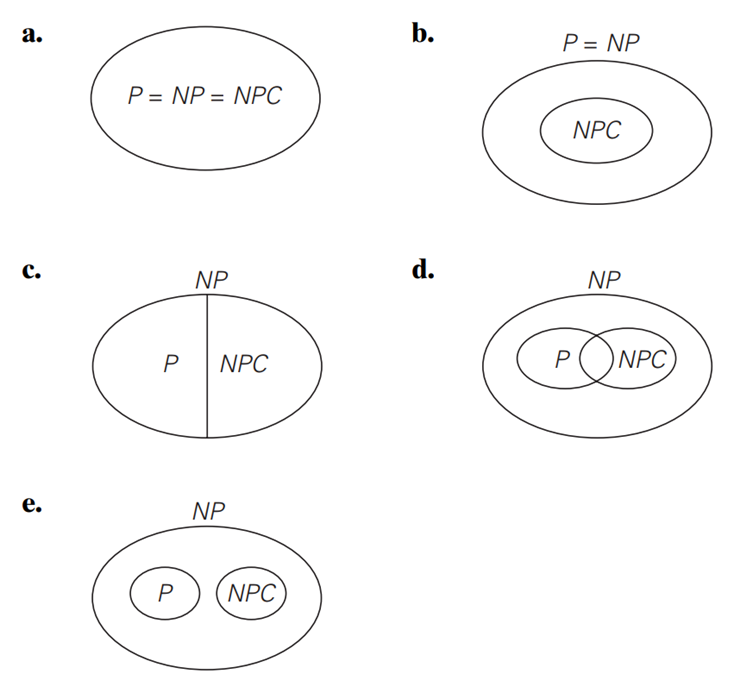
\includegraphics[scale = 0.5]{Picture.png} \\
\end{center}
The diagram \textbf{e} does not contradict the current state of our knowledge according to Ladner's theorem. P is set of problems that can be solved by a deterministic Turing Machine in polynomial time. NP is set of decision problems that can be solved by Non-deterministic Turing Machine in polynomial time. Note that P is subset of NP ($P \subset NP$). Thus $a$ and $b$ can't be an answer. Informally, NP is set of decision problems which can be solved by a polynomial time via a "Lucky Algorithm", a magical algorithm that always makes a right guess among the given set of choices. $c$ can't be an answer too since there are some problems neither part of P and not part of NPC. When we look at $d$, we can see that $d$ is wrong if P and NPC are overlapped, then it should be completely overlapped. It's impossible to be partially disjoint. Thus the answer is \textbf{e}.

\end{document}